\documentclass[11pt, journal,letterpaper,compsoc]{IEEEtran}
%\usepackage{cite}
\usepackage{graphicx}
\usepackage{caption}
\usepackage{refstyle}

% correct bad hyphenation here
\hyphenation{op-tical net-works semi-conduc-tor}


\begin{document}

\title{Diamer Bhasha Dam: A Successful Project or A Fraud?}

% As a general rule, do not put math, special symbols or citations
% in the abstract
\IEEEtitleabstractindextext{%
\begin{abstract}
A dam is a barrier/great wall that stops or store the flow of water or underground streams. A dam can also be used to save water or for storage of water which can be evenly distributed for irrigation, human consumption, industrial use, agricultural use, and navigability. Main purpose of the dams is to retaining water, while other structures like floodgates have the purpose to prevent water flow into land regions.
As per recent research studies, In the coming future (Approx. 2025) Pakistan will face water shortage due to rapid increase in the country’s population and misuse of water throughout the country. To overcome the water shortage issue Pakistan needs to build more dams to store water such as Diamer Bhasha dam which is one of the largest dams in Pakistan which will not only store water but will also generate 4,500 MW of electricity to the national grid, so it can also reduce the shortage of electricity in the country as well. Diamer Bhasha dam which is named after Diamer (a district in northern areas of Pakistan called Gilgit Baltistan) and Bhasha (a village in Kohistan in the province of Khyber Pakhtunkhwa).
\end{abstract}

\begin{IEEEkeywords}
DAM, Water.
\end{IEEEkeywords}
}


% make the title area
\maketitle
\IEEEdisplaynontitleabstractindextext


\IEEEpeerreviewmaketitle

\section{Introduction}
\IEEEPARstart{D}{iamer-Basha}  dam was started by Government of Pervez Musharraf in 2008.The project is located on Indus River, about 315 km upstream of Tarbela Dam, 165 km downstream of the
Northern Area capital Gilgit and 40 km downstream of Chilas at Basha Distt. Diamer Gilgit- Baltistan. It will have height of 272 meter with 7.9 km3 annual surface face water capacity. However, the location of dam is in disputed area hence no country or organization is willing to
loan \$12 billion for construction of this dam without NOC from India. Pakistan has to construct this dam from its own resources.

\begin{figure} 
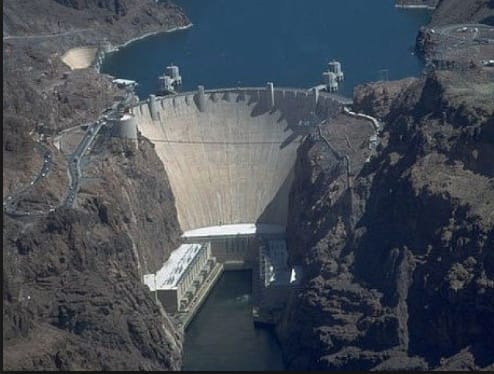
\includegraphics[width=\linewidth]{images/dam}
\caption{Dam Site}
\label{fig:dam}
\end{figure}


The planned 4,500 MW Diamer-Bhasha Dam on the Indus in Pakistan is, at US\$12.6 billion (2008), one of the largest and most costly planned dams in the world. A huge amount of Rs 27.824 billion is allocated for the acquisition of land and resettlement of the people living in the nearby area’s that will be affected in the wake of the construction of the dam. Diamer bhasha dam will have water storage capacity of 8,100,000-acre feet (10.0 km3). 



In August 2012,the project faced several setbacks due to major sponsors backing out from financing the project, as World Bank and Asian Development Bank both refused to finance the project as according to them its location is in disputed territory and asked Pakistan to get
 a NOC from neighboring India.
\hfill  

In August 2013,Finance Minister of Pakistan: Claimed to have convinced the World Bank and The Aga Khan Development Network to finance the Diamer-Bhasha Project without the requirement of NOC from India. Asian Development Bank, Aga Khan Rural Support Programme
 (AKRSP) and Aga Khan Foundation had agreed to become lead finance manager for the project.
\hfill  

On November 7, 2013, the Chairman of WAPDA :Syed Raghib Abbas Shah claimed that his department has received 17,000 acres of land at the cost of Rs 5.5 billion from Government of Gilgit-Baltistan and the Ismaili Community for the construction of the project.
\hfill 
 
In November 2017,Pakistan dropped its bid to have the dam financed under the China-Pakistan Economic Corridor (CPEC) framework as China placed strict conditions including on the ownership of the project. China had projected the cost of the dam to be \$14 billion and for
securitization of its, investment China wanted Pakistan to pledge another operational dam to it.
\hfill 


\section{Understanding the need of DAM in Pakistan}
Water is essential for life and sadly Pakistan is facing sever water crisis. The UNO has listed Pakistan 7th in the list of countries facing water crisis. The consumption of water is much bigger than its supply. The growth rate of Pakistan’s population is 5.7, so after a few years the population will multiply but I think water supply will not be matching with the population increase. Will we be able to accommodate our people basic necessity?
Pakistan is a country where water is wasted in floods but no dams or reservoirs are built. Different areas in Pakistan receive a vast amount of rainfall but all water drains down by improper planning of saving that water for meeting the needs of our country. Pakistan being an agriculture country has a dire need of water. It will come as a shock, but only two dams have been made in the past 70 years.

 
 \section{Construction Time And Budget}
Diamir Bhasha dam is expected to start in April 2020 (1/5 land still to be acquired for reaching total required of 37500 Acres) and Bhasha Dam expected Completion is in 9 (Nine) years i.e. Apr 2029.
Mohmand Dam is expected to start in April 2019 and its expected Completion is in 6 years i.e. by 2025.

The planned 4,500 MW Diamer-Bhasha Dam on the Indus in Pakistan is, at US\$12.6
billion, one of the largest and most costly planned dams in the world. In August 2008,
a fact-finding team visited the proposed site of the dam for one week to collect
information and document the public perception of the project. The team was
composed of four Pakistani water experts: Mr. Mustafa Talpur, Mr. Ifthikhar Hussain
and Mr. Mohsin Babbar and Mr. Aimal Khan from Sungi Development Foundation.
Ms. Sameeta Ahmad, Assistant Professor, Department of Architecture, NWFP UET,
Abbottabad Campus, and Member of the Pakistan Chapter of the International
Council on Monuments and Sites (ICOMOS) assisted the team by giving her input on
questions related to cultural heritage.
Dams built for energy, irrigation, and drinking water. Dams however, are not built without a significant cost. After a prolonged delay, Pakistan gave go-ahead for the establishment of Diamer-Bhasha dam at an initial cost of Rs625 billion.
The funding for the Diamer-Bhasha dam would be arranged via local resources since international lending entities and China hesitated in assisting the country build the dam, reported Express Tribune. The Ministry of Planning and Development said the Central Development Working Party (CDWP) had given go-ahead for clearance of Diamer-Bhasha Dam project by the Executive Committee of National Economic Council (ECNEC). Diamer-Bhasha dam would only be setup as a water reservoir and doesn’t include power generation side, which would cost an additional Rs744 billion. The total cost of Diamer-Bhasha dam at the minimum would be Rs1.4 trillion once the power generation facilities are factored in. The money for this project would be provided from the budget by the government and Water and Power Development Authority (WAPDA) would organize commercial funding, Sartaj Aziz said. The money for this project would be provided from the budget by the government and Water and Power Development Authority (WAPDA) would organize commercial funding, Sartaj Aziz said. Around Rs48 billion a year would need to be provided for the building of the dam. Federal government will give Rs370.2 billion from the budget as a grant, which will translate into 57 percent of the construction cost. And Wapda would raise over Rs115.9 billion via various sources as equity investment and authorities will obtain Rs163.3 billion in commercial loans, as per the project document. Out of the total Rs625 billion cost of building Diamer-Bhasha dam, it will have interest during construction, local rupee share would be Rs472 billion and Rs153.2 billion foreign exchange components to be obtained from overseas. Completion period is set to be five years. Rs138 billion has been reserved for land acquisition, resettlement and majority of this work has been carried out. The authorities have spent over Rs58.3 billion on land purchase in the area and Rs53.5 billion has also been endorsed for resettlement.

\section{Location}
The project is located on Indus River,about 315 km upstream of Tarbela dam,165 km downstream of the northern area capital Gilgit and 40 km downstream of chilas.
\begin{figure}  [h!]
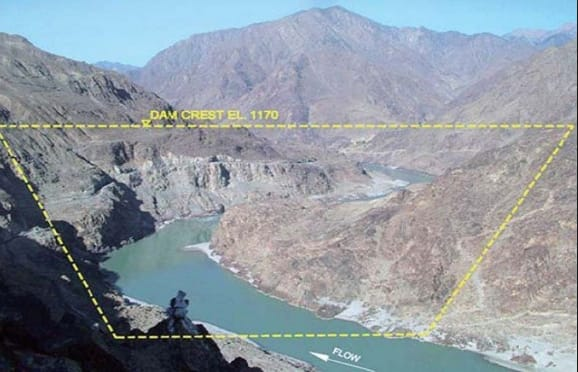
\includegraphics[width=\linewidth]{images/dam-location}
\caption{Dam Location}
\label{fig:dam1}
\end{figure}

\section{Details}
\begin{figure}  [h!]
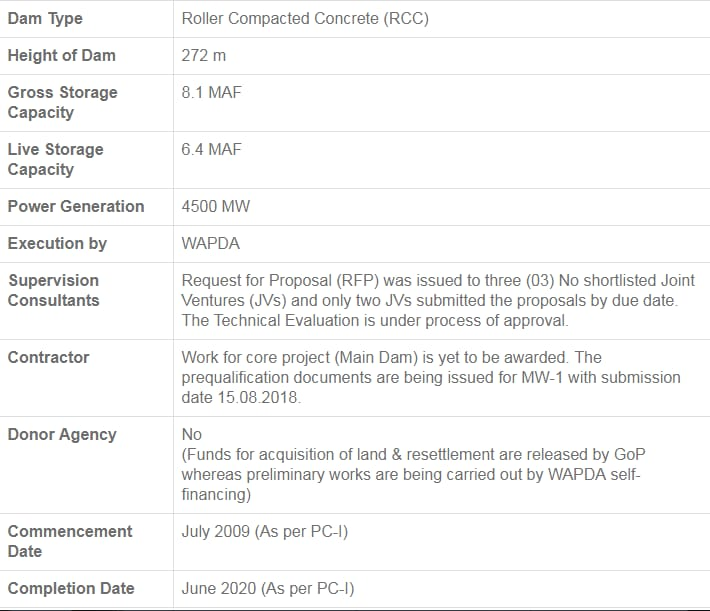
\includegraphics[width=\linewidth]{images/detail}
\caption{Details}
\label{fig:dam2}
\end{figure}

 \section{Income Sources}
 As mentioned above that world bank and Asian development bank backed out from funding the project and no other international investors are investing in the particular project. This means Pakistan will need to fund the project from its local sources, however local banks and financial organizations will not be able to meet the required fund for the constructions for the project. This is why Chief justice of Pakistan (CJP) launched a fundraising campaign for the project, this campaign will have great impact on the people of Pakistan regarding the importance of water that is being misused and safe as much water as they can. This campaign will unite the people of Pakistan for a national cause which will secure the future for coming generation.

\subsection{Online Transaction fund}
In order to fund through online transaction fund for the project an account is created in the state bank of Pakistan with the account name: THE SUPREME COURT OF PAKISTAN AND THE PRIME MINISTER OF PAKISTAN DIAMER-BHASHA AND MOHMAND DAMS FUND and account no: 03-593-299999-001-4 Which was created on 6th of July 2018 and the amount which has been funded by the great people of Pakistan is Rs. 7,903,605,048 (Seven billion nine hundred three million six hundred five thousand forty-eight rupees) till 22nd of November 2018.

\subsection{SMS}
Alternatively, you can also make small contributions as low as Rs. 10 to the Supreme Court Dam fund by sending SMS from mobile phones.
	
	\begin{itemize}
		\item The user shall type “dam”. 
		\item Send SMS to 8000. 
	\end{itemize}

The user will also receive a confirmation message with gratitude.


\subsection{CJ/PM Fund, International Fund Raising Trip}
Keeping in view the need to construct dams and reservoirs in Pakistan, Chief Justice of Pakistan (CJP) Saqib Nisar has created  Supreme Court of Pakistan – Diamer Bhasha and Mohmand Dams – Fund . There are various personalities who have contributed to it; some others from various walks of life are willing to do so. The fund was established on July 4 with an ambition to eradicate water crisis from the country. Masses’ participation in the fund can be done if they send an SMS by typing ‘dam’ and sending it to 8000, charges are Rs10 on each message. Diamer Bhasha Dam Fund has now reached Rs 3.33 billion. Until Sep 7, the country wise data showed that within Pakistan an amount of Rs 1,972,643,520 (Rs1.97 billion) was collected through bank branches, interbank transfers and mobile phone SMS service. Out of total donation received from within the country, amount collected through debit/credit cards stands at Rs 122 million, Rs 65.8 million were collected through SMS service, Rs 65.5 million from Interbank transfer service whereas an amount of Rs 2.95 billion was collected at bank branches. The Fund has been established by the SBP on the directions of the Supreme Court. All the commercial and micro-finance banks, and field offices of SBP Banking Services Corporation have opened the Fund account to receive donations in cash, and through cheques, pay orders and demand drafts at all their branches across the country.

\subsection{Loan}
The authorities will borrow Rs163.3 billion in commercial loans

\subsection{Govt Budget}
The federal government will provide Rs370.2 billion from the budget in a grant, which will cover 57\% of the cost. 

\subsection{Wapda}
Wapda will raise Rs115.9 billion from its own sources as an equity investment.

\subsection{Provincial Govt}
Replace the sample Text here.

\subsection{Pakistan Railway train service}
Replace the sample Text here.

\subsection{Salary of Govt Employees}
Replace the sample Text here.

\subsection{Tax on Bills}
Replace the sample Text here.
	

\section{Consideration}

\subsection{Access Information}
Transparency levels in Pakistan are generally poor and it is very difficult to get access to information about any development project, program or policy. The fact finding team learned that the same was true for the Diamer-Bhasha dam. In numerous meetings of the fact finding team with project-affected people, officials of the district administration and the execution agency, the team learned that planners, designers and the execution agency had never consulted stakeholders of the project. Some representatives of the people who will be displaced by the project told the fact-finding team that the only visits they had received in connection with the project were from private consultants who had come to assess the size and value of the land. Contrary to the relevant laws, no public hearing was organized after conducting the Environmental Impact Assessment. 

\subsection{Environmental Impact}
1. Villages affected: 31 \\
2. Houses affected: 4,100 \\
3. population affected: 35,000 \\
4. Agricultural land submerged: 1,5000 acres \\
5. Area under reservoir: 25,000 acres 

\subsection{Resettlement}
 1. Proposed new settlements: 9 model villages  \\
 2.  Population resettled: 28,000 \\
 3. New infrastructure, roads, clean water supply schemes, schools, health centres, electricity supply, etc. \\ 
 4. Development of new tourism industry in area around reservoir (including hotels, restaurants, water sports, etc.) \\
 5. Development of hitherto non-existent fresh-water fishing industry based on newly created reservoir \\

\subsection{Currency Devaluation}
If the dam project starts in 2020, then it is expected to complete by 2029. Asian region is developing continuously which is the reason why concrete demand is going to increase in next decade. Because of demand-supply gap, concrete price is going to soar. Pakistan also needs to pay outstanding liability of 92 billion dollars in next decades. Due to this Pakistan’s economy is not going to get boom till 2030.

\begin{figure}  [h!]
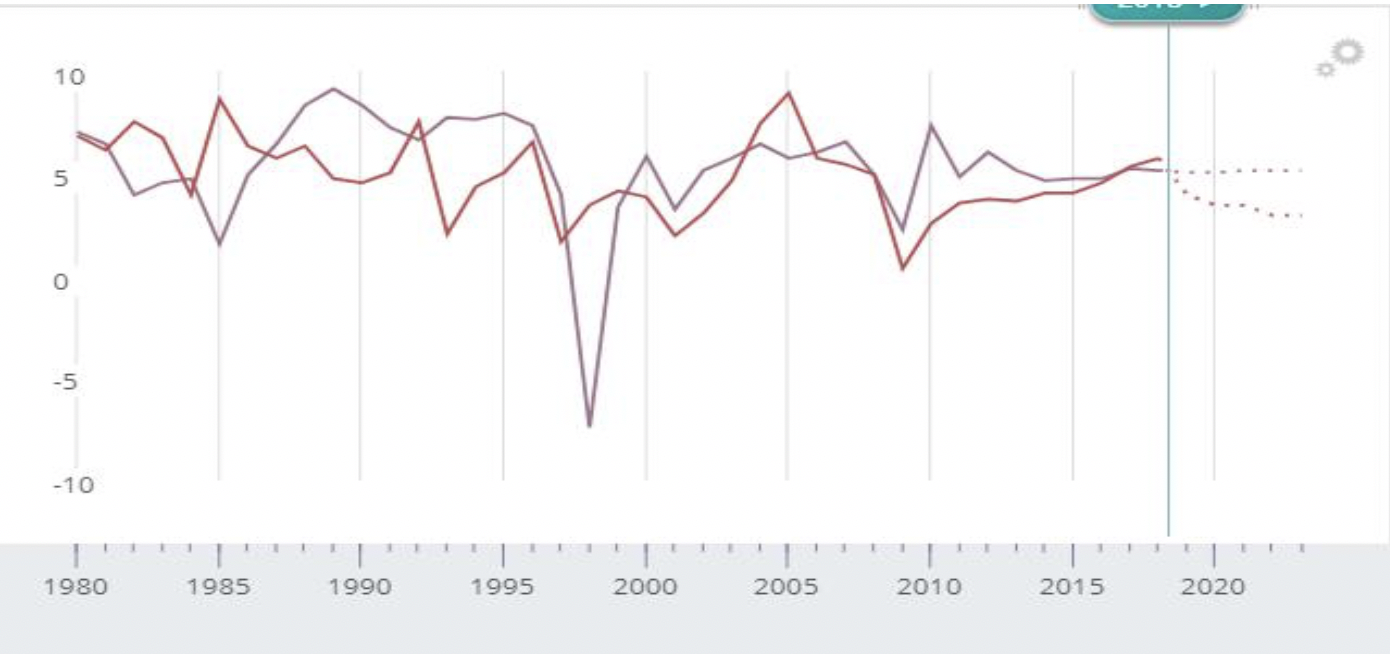
\includegraphics[width=\linewidth]{images/pak-vs-asia}
 \caption{Pakistan VS South-East Asia}
% \label{fig:dam3}
\end{figure}

By the end of 2029 Pakistan will need more of 1 billion dollars for project completion and hence  total estimated cost will rise to 14.1 billion dollars.\\

\begin{figure}  [h!]
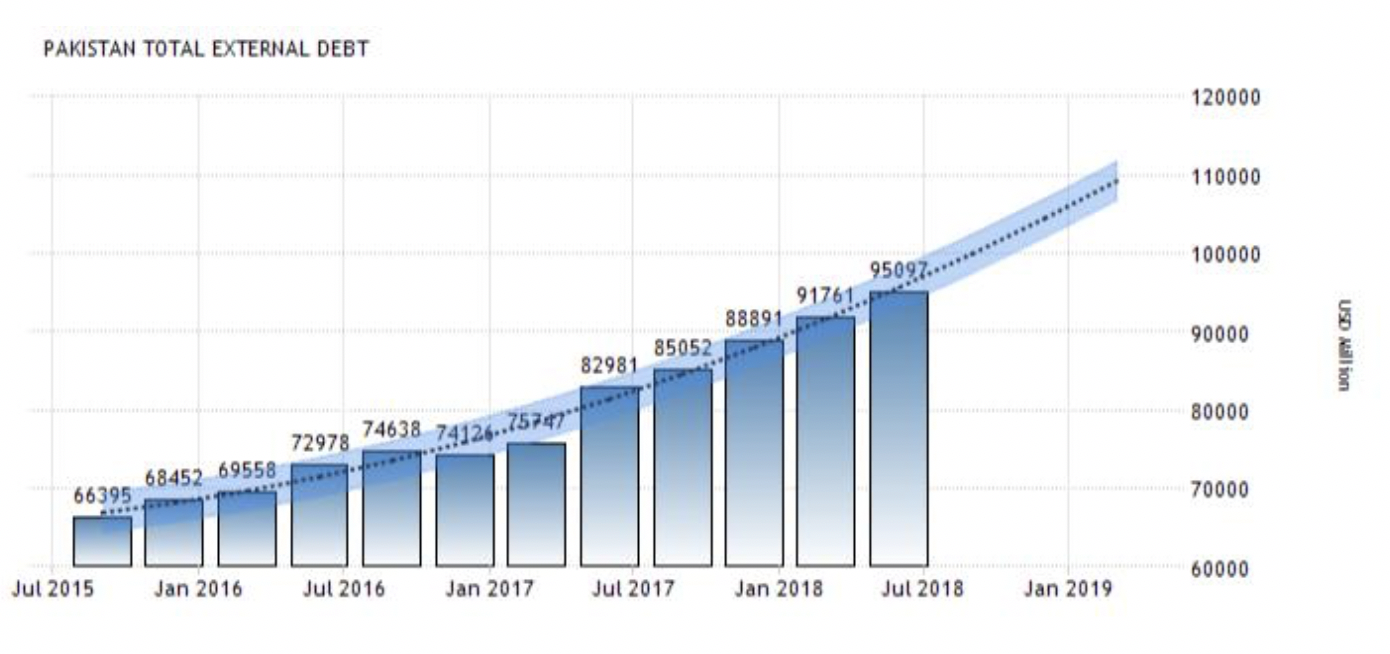
\includegraphics[width=\linewidth]{images/predicted-gdpa}

% \label{fig:dam3}
\end{figure}

The graph below shows the predicted GDPA of Pakistan by IMF. \\
\begin{figure}  [h!]
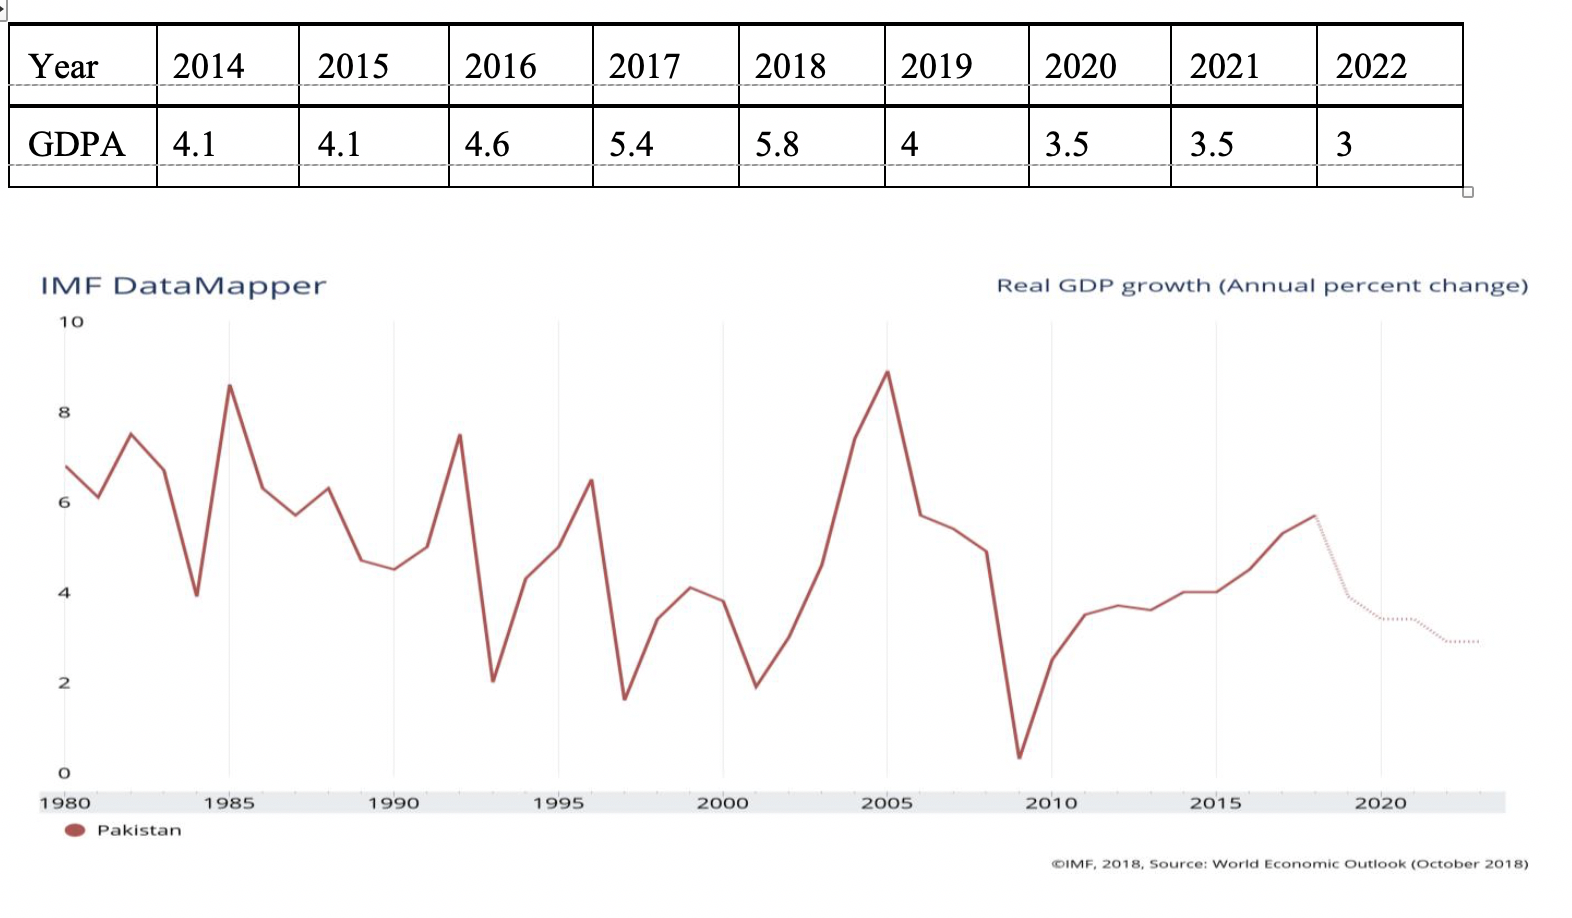
\includegraphics[width=\linewidth]{images/gdpa-imf}
 \caption{Predicted GDPA of Pakistan by IMF}
% \label{fig:dam3}
\end{figure}

\subsection{Forecast Data}

The Graph below  shows Fund Raising Status for The Supreme Court of Pakistan and Prime Minister of Pakistan Diamer-Bhasha and Mohmand Dam Funds.\\ 

\begin{figure}  [h!]
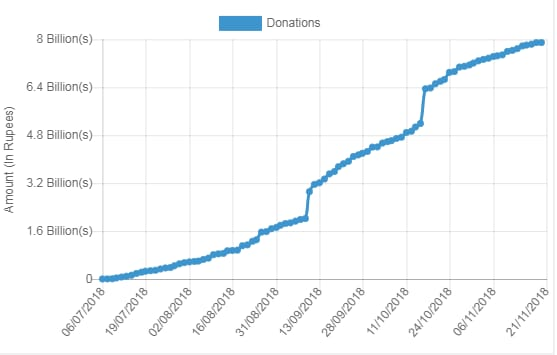
\includegraphics[width=\linewidth]{images/fund-status}
 \caption{Fund Raising Status for Diamer Bhasha Dam}
% \label{fig:dam3}
\end{figure}

\section{Conclusion}
Although Chief Justice of Pakistan's sensitivity to growing water crisis in Pakistan is appreciable but this is not the way infrastructure finance is done.You do not crowd-source a mega dam.\\
A few questions arises when trying to use voluntary donations to fund the Diamer-Bhasha Dam.\\
1) From a briefing given by water and power officials at a hearing of the Senate Standing Committee on Planning, Development and Reform the cost of dam has been given as Rs1.450 trillion.The total amount deposited in Dam fund account till now is Rs 7 billion.
Now lets assume that on average, the account sees an inflow of Rs20m per day (which is highly optimistic), then it will take 72,500 days to reach the target, or 199 years.\\
2) Take a look at another angle.According to Public Sector Development Programme (PSDP) document on the Planning Commission’s website, for next year, the amount allocated for construction of the dam part of the project alone is Rs23.68bn .If it is so,
then at Rs20m per day, it will take 1,184 days to reach the target of Rs23.68bn, or 3.2 years which means even next year’s PSDP allocation (for the dam part alone) will not be possible to meet the amount. \\
3) Now assume a different situation. Lets say the contributions for dam comes as doubles in size that means time period will reduce to half.Now lets assume that instead to pay for the entire dam the contributions are meant only to supplement government allocations for the project. Even then, a year’s intake of Rs7.3bn (assuming a Rs20m per day average contribution for the year) will not even be enough to pay for a portion of the resettlement cost of the project. \\
Public finance is not a joke.The state cannot be run like a charity also the infrastructure finance cannot be crowd-sourced like this.People have rights to ask a few basic questions before they are asked to contribute their hard-earned money like What will this money be used for? Who will have the authority to transact these funds? What rules will govern its distribution? How much of an impact will my contribution have? Authorities need to answer these questions first.
\section*{Recommendations}
1) Sources  have said that the government was considering to burdening the rich instead of the poor to construct the dam. Imposition of a tax on bridges, barrages, and on inter-provincial crossing to collect amount for the dam would be a good step.  \\
2) Government can form company named "Diamer-Bhasha Private limited"  and then market the shares of this company by keeping approximately 51 to 53 percent shares of company. After that a campaign is needed to be launch eplaining how investors can be benefitted from it.\\
3) Government can also encourage Pakistnis to contribute in Dam fund by relieving them in their monthly utility bills.
\\

\begin{thebibliography}{1}
%\bibliographystyle{IEEEtran}
%\bibliography{references}
\bibitem{IEEEhowto:kopka}


\end{thebibliography}




% that's all folks
\end{document}


